\documentclass[twocolumn]{article}
\usepackage[english]{babel}
\usepackage[utf8]{inputenc}
\usepackage{amsmath,amssymb,physics,mathtools,blindtext,graphicx,float}
\usepackage[a4paper,total={7.5in,10in}]{geometry}
\usepackage[labelfont=bf]{caption}

\begin{document}
\begin{large}
\begin{equation}
    \label{26apr0749}
    \left(-\frac{\hbar^2}{2\mu}\frac{\text{d}^2}{\text{d}r^2} + \frac{\hbar^2\ell(\ell+1)}{2\mu r^2} - \frac{Ze^2}{4\pi\epsilon_0r}\right)P_{n\ell}(r) = EP_{n\ell}(r).
\end{equation}

\subsection*{Numerical solution}
The following dimensionless variables were defined:
\begin{equation}
    \begin{split}
        &\xi = r/Da_0 \\ 
        &E' = E/\left(Z^2\mu\hbar^2/(2m_e^2a_0^2)\right)
    \end{split}
\end{equation}
In principle, $E'$ should take the values $-1,-1/4,-1/9,\dots$ for bound states. The variable $\xi$ is on the interval $[0,1]$ and $D$ is chosen so that the wavefunction is negliably small in the vicinity of $\xi=1$. Using these variables, equation \eqref{26apr0749} can be written
\begin{equation}
    \label{20apr0705}
    \hat{H}u = -\beta^2\left(\frac{\text{d}^2}{\text{d}\xi^2}-\frac{\ell(\ell+1)}{\xi^2}+\frac{2}{\beta\xi}\right)u = E'u
\end{equation}
where $\beta = m_e/(Z\mu\alpha)$. The numerical solution to \eqref{20apr0705} is written as a linear combination of $n$ B-splines of degree $k$:
\begin{equation}
    \hat{u}(\xi) = \sum_{j=0}^{n-1}c_jB_{j,k}(\xi).
\end{equation}
The boundary conditions $u(0) = u(1) = 0$ are satisfied by placing multiple knot points at $\xi=0$ and $\xi=1$. This makes $B_{0,k}$ the only non-zero B-splines at $\xi=0$ and $B_{n-1,k}$ the only non-zero B-spline at $\xi = 1$. Since the wavefunction is vanishing for $\xi$ closer to one, it becomes more efficient to place distribute the knot points unevenly over $[0,1]$ such that there are more of them closer to zero than closer to one. The knots were thus placed according to the function $2^{x^2}-1$ where $x\in(0,1)$. 

so that closer to zero than closer to oneThe boundary conditions are thus satisfied by setting $c_0=c_{n-1}=0$. Inserting this into equation \eqref{20apr0705}, multiplying by $B_{i,k}(x)$ and integrating over $(0,1)$ yields:
\begin{equation}
    \sum_{j=1}^{n-2}c_j\int\limits_0^1B_{i,k}\hat{H}B_{j,k} = E'\sum_{j=1}^{n-2}c_j\int\limits_0^1B_{i,k}B_{j,k}
\end{equation}
which is a generalized eigenvalue problem of the form $A\mathbf{c} = E'B\mathbf{c}$. This is solved with a inverse power method, $(A-E^*B)\mathbf{c}_{j+1} = B\mathbf{c}_j$ where $E^*$ is a guess at an eigenvalue and $\mathbf{c}_j$ is normalized in each iteration.



\subsection*{Results}
\begin{table}[!b]
\centering
\begin{tabular}{c c c}
    $n$ & $\ell$ & $|E'-1/n^2|$ \\ 
    \hline\hline
    1 & 0 & $1.7\cdot 10^{-3}$ \\ 
    2 & 0 & $4.2\cdot 10^{-4}$ \\ 
    2 & 1 & $1.1\cdot 10^{-9}$ \\ 
    3 & 0 & $1.8\cdot 10^{-4}$ \\ 
    3 & 1 & $1.2\cdot 10^{-7}$ \\  
    3 & 2 & $3.5\cdot 10^{-8}$ \\ 
    4 & 0 & $1.0\cdot 10^{-4}$ \\ 
    4 & 1 & $2.6\cdot 10^{-6}$ \\ 
    4 & 2 & $1.2\cdot 10^{-6}$ \\ 
    4 & 3 & $2.7\cdot 10^{-7}$
\end{tabular}
\caption{}
\end{table}
\begin{figure}[!t]
    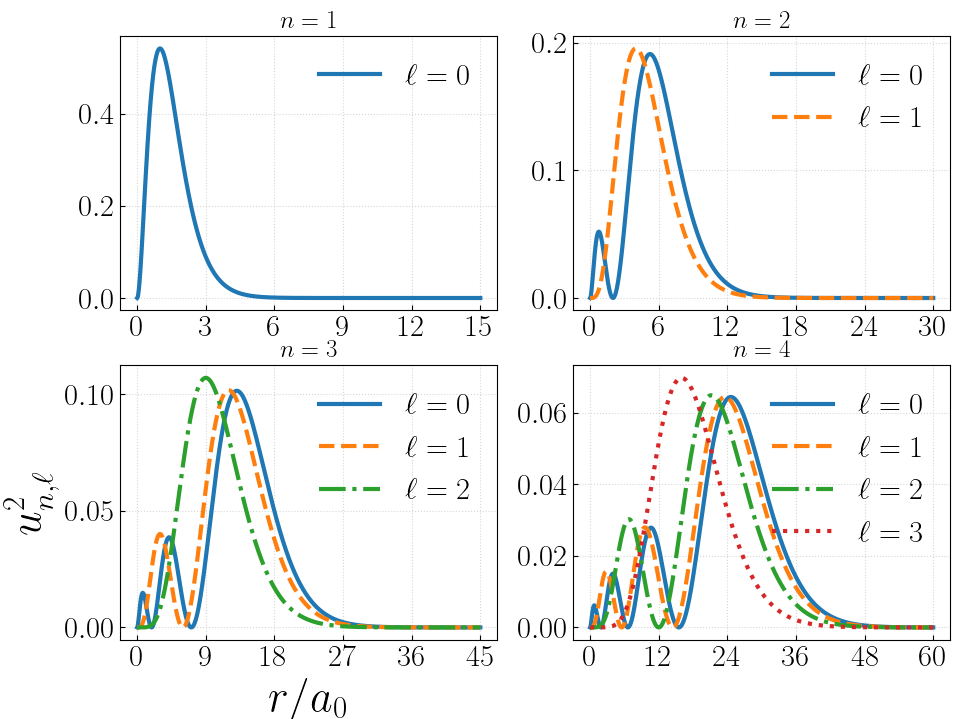
\includegraphics[scale=0.4]{Hatom.png}
    \caption{}
\end{figure}


















\end{large}
\end{document}
